%\documentclass[preview]{standalone}
\documentclass[pagesize,paper=a4]{scrartcl}
\usepackage{pdflscape}
\usepackage{smartdiagram}
\usepackage{tabularray}
\usepackage{chemfig}
\usepackage{chemmacros}
\usepackage{siunitx}
\chemsetup{modules={all}}
\chemsetup[redox]{pos=top,roman=false}
\chemsetup[redox]{pos=top}
\chemsetup{redox/sep=.5em}
\chemsetup[redox]{explicit-sign=true}
\usepackage[tikz]{bclogo}
%\usepackage{mol2chemfig}
%\usepackage{pst-blur}
\usepackage[edges]{forest}
\usepackage{amsmath,amssymb,braket,tikz}
\usetikzlibrary{fit,patterns,shadows.blur,shapes,mindmap}
\usetikzlibrary{arrows,arrows.meta,decorations.markings,shapes.symbols}
\usetikzlibrary{decorations.pathreplacing, decorations.pathmorphing,calc,arrows,positioning,tikzmark}
\usetikzlibrary{bending}

\NewTblrTheme{fancy}{
	\SetTblrStyle{firsthead}{font=\bfseries}
	\SetTblrStyle{firstfoot}{fg=blue2}
	\SetTblrStyle{middlefoot}{\itshape}
	\SetTblrStyle{caption-tag}{red2}
}

\usepackage{empheq}
\setchemfig{fixed length=false, atom sep=2.5em, arrow offset=6pt, scheme debug=true}
\usepackage[most]{tcolorbox}
\usepackage[dvipsnames]{xcolor}


\pgfdeclarelayer{background}
\pgfsetlayers{background, main}


\begin{document}
\KOMAoptions{pagesize,paper=landscape,DIV=20}

\begin{center}

\scalebox{.87}{
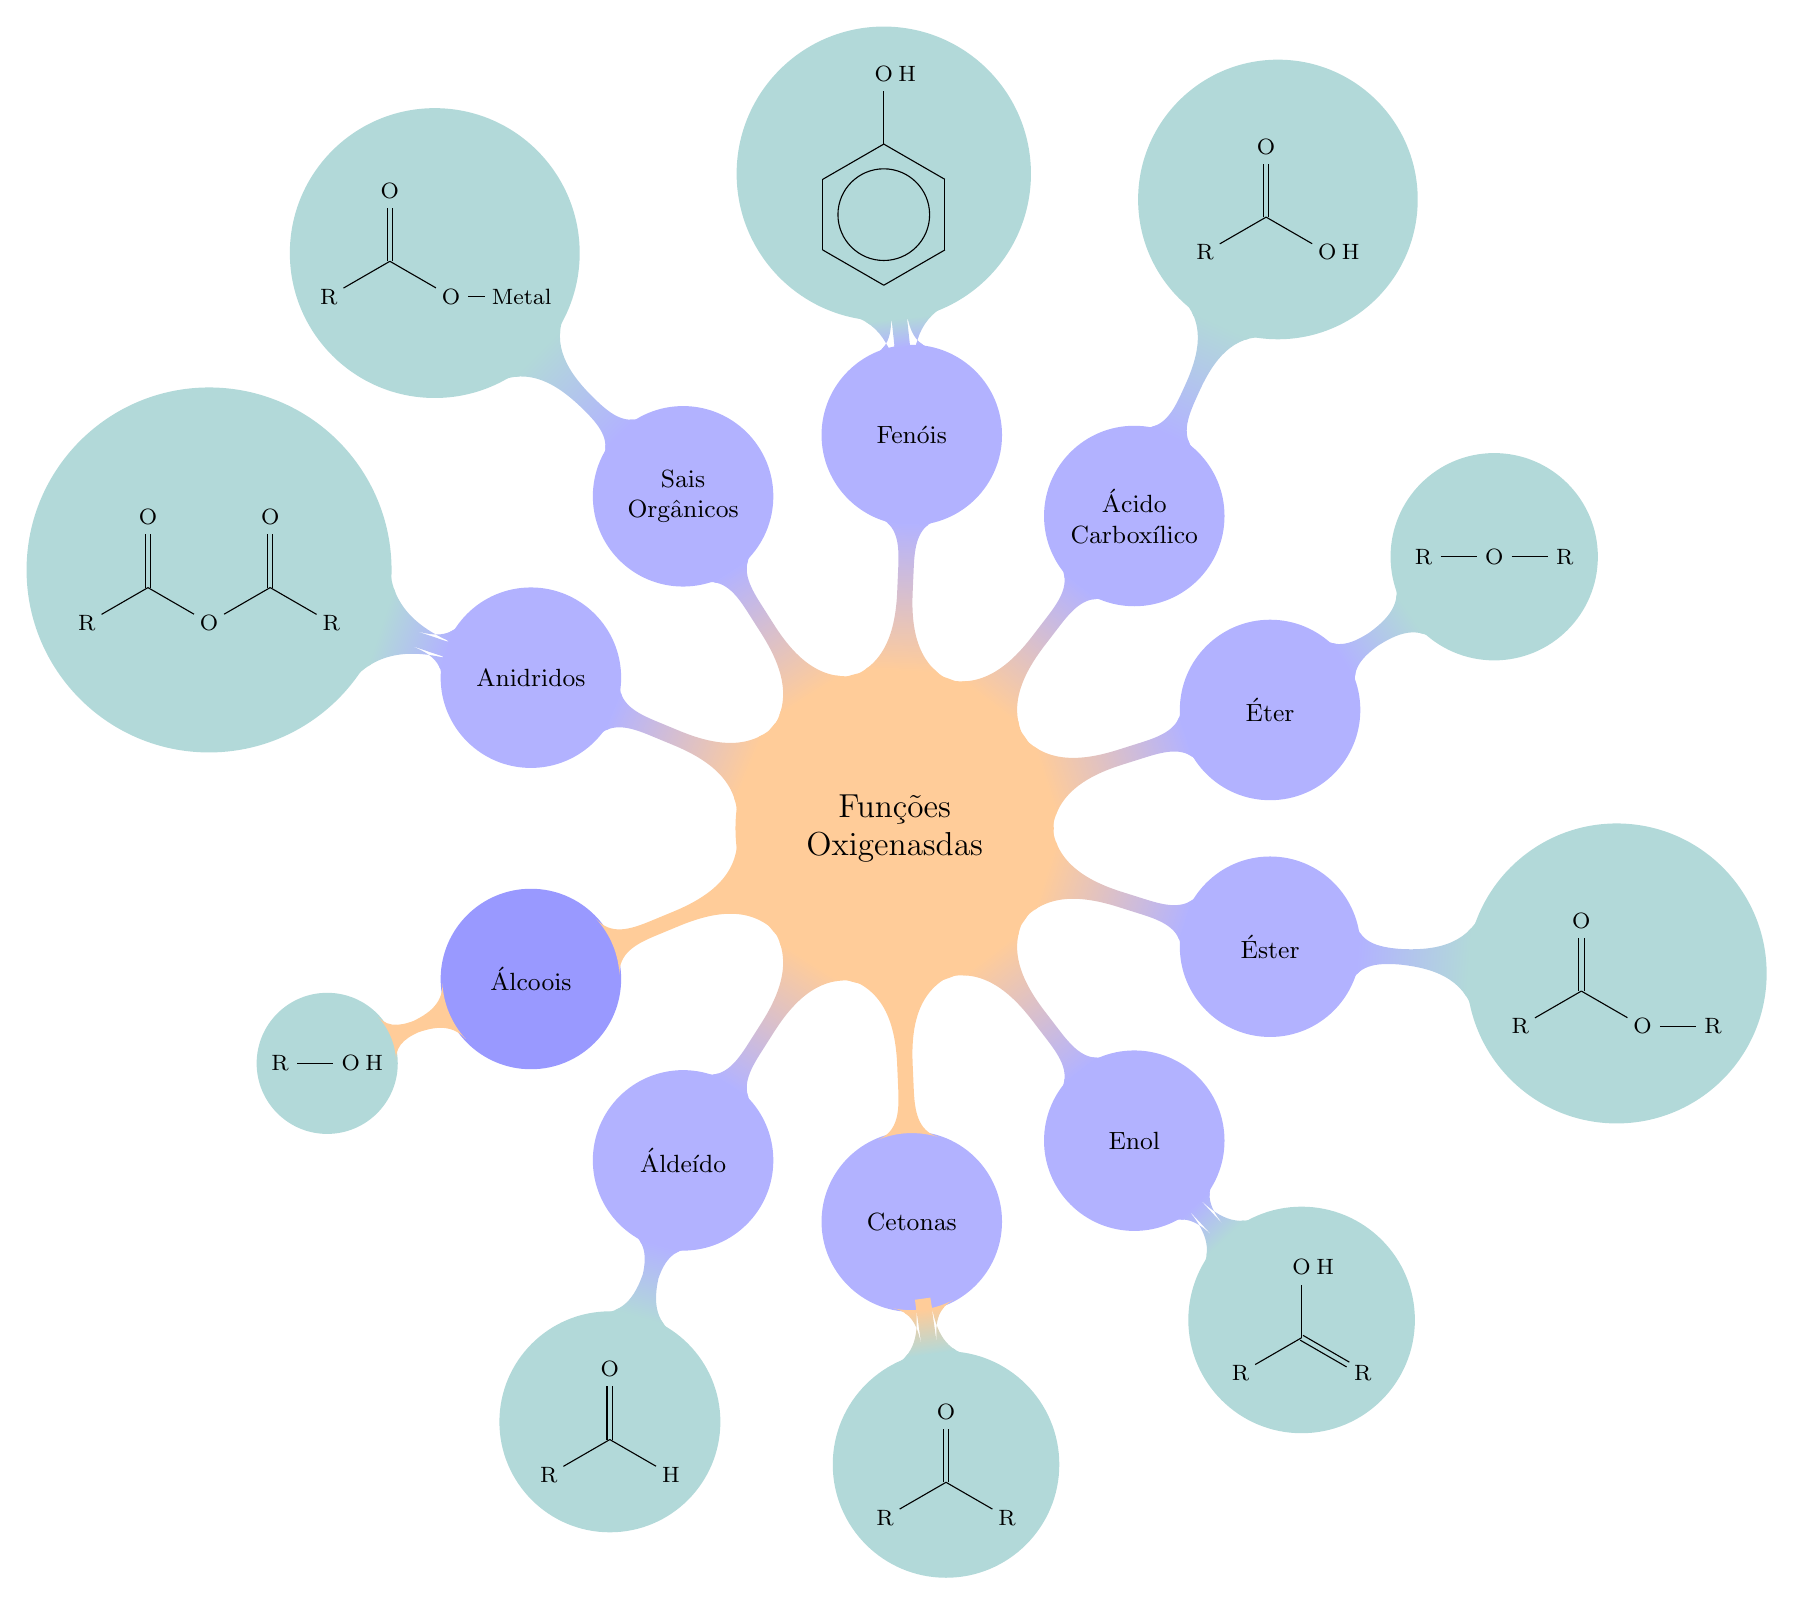
\begin{tikzpicture}[mindmap, grow cyclic, every node/.style=concept, concept color=orange!40, 
	level 1/.append style={level distance=5cm,sibling angle=35},
	level 2/.append style={level distance=2.8cm,sibling angle=90},]

	\node {Funções \\ Oxigenasdas}
	child {node [concept color = blue!40] {Álcoois}
		child {node [concept color = teal!30] {\chemfig{R-OH} \\ }}
	}
	child [concept color = blue!30] {node {Áldeído}
			child [concept color = teal!30, xshift=.5cm, yshift=1cm, text width=2.1cm,] {node {\chemfig{R-[:30](=[:90]O)-[:330]H}}}
	}
	child {node [concept color = blue!30] {Cetonas}
		child [concept color = teal!30, xshift=.3cm, yshift=.3cm, text width=2.2cm] {node {\chemfig{R-[:30](=[:90]O)-[:330]R}  }}
	}
	child [concept color = blue!30] {node {Enol}
		child [concept color = teal!30, xshift=.3cm, yshift=.3cm, text width=2.2cm] {node {\chemfig{R-[:30](-[:90]OH)=[:330]R}  }}
	}
	child [concept color = blue!30] {node {Éster}
				child [concept color = teal!30, xshift=1.5cm, yshift=1cm, text width=3.3cm] {node {\chemfig{R-[:30](=[:90]O)-[:330]O-R}}}
	}
	child [concept color = blue!30] {node {Éter}
				child [concept color = teal!30,xshift=.5cm, yshift=1cm, text width=2.5cm] {node {\chemfig{R-O-R}}}
	}
	child [concept color = blue!30] {node {Ácido \\ Carboxílico}
				child [concept color = teal!30, xshift=1.5cm, yshift=1cm, text width=3.cm] {node {\chemfig{R-[:30](=[:90]O)-[:330]OH}}}
	}
	child [concept color = blue!30] {node {Fenóis}
				child [concept color = teal!30, xshift=.5cm, yshift=.5cm, text width=2.2cm] {node {\chemfig{**6(----(-OH)--)}  }}		
	}
	child [concept color = blue!30] {node {Sais \\ Orgânicos}
				child [concept color = teal!30, xshift=1.5cm, yshift=1cm, text width=3.cm] {node {\chemfig{R-[:30](=[:90]O)-[:330]O-Metal}}}
	}
	child [concept color = blue!30] {node {Anidridos}
				child [concept color = teal!30, xshift=1.5cm, yshift=.3cm, text width=4.2cm] {node {\chemfig{R-[:150](=[:90]O)-[:210]O-[:150](-[:210]R)=[:90]O}}}
};
\end{tikzpicture}
}
\end{center}

\begin{tikzpicture}
\node[draw=none,red,text width=7cm,font={\large\bfseries}] at (0,3) {Funções Oxigenadas}; 	
 \node[draw=none,text width=7cm,font={\large\bfseries}] at (20,3) {Prof. Fábio Lima};
\end{tikzpicture}

\KOMAoptions{paper=a4,paper=portrait,DIV=10}

\end{document}

